\documentclass[]{article}
\usepackage{lmodern}
\usepackage{amssymb,amsmath}
\usepackage{ifxetex,ifluatex}
\usepackage{fixltx2e} % provides \textsubscript
\ifnum 0\ifxetex 1\fi\ifluatex 1\fi=0 % if pdftex
  \usepackage[T1]{fontenc}
  \usepackage[utf8]{inputenc}
\else % if luatex or xelatex
  \ifxetex
    \usepackage{mathspec}
  \else
    \usepackage{fontspec}
  \fi
  \defaultfontfeatures{Ligatures=TeX,Scale=MatchLowercase}
\fi
% use upquote if available, for straight quotes in verbatim environments
\IfFileExists{upquote.sty}{\usepackage{upquote}}{}
% use microtype if available
\IfFileExists{microtype.sty}{%
\usepackage{microtype}
\UseMicrotypeSet[protrusion]{basicmath} % disable protrusion for tt fonts
}{}
\usepackage[margin=1in]{geometry}
\usepackage{hyperref}
\PassOptionsToPackage{usenames,dvipsnames}{color} % color is loaded by hyperref
\hypersetup{unicode=true,
            pdftitle={Session regression I: simple linear regression},
            colorlinks=true,
            linkcolor=Maroon,
            citecolor=Blue,
            urlcolor=blue,
            breaklinks=true}
\urlstyle{same}  % don't use monospace font for urls
\usepackage{color}
\usepackage{fancyvrb}
\newcommand{\VerbBar}{|}
\newcommand{\VERB}{\Verb[commandchars=\\\{\}]}
\DefineVerbatimEnvironment{Highlighting}{Verbatim}{commandchars=\\\{\}}
% Add ',fontsize=\small' for more characters per line
\usepackage{framed}
\definecolor{shadecolor}{RGB}{248,248,248}
\newenvironment{Shaded}{\begin{snugshade}}{\end{snugshade}}
\newcommand{\AlertTok}[1]{\textcolor[rgb]{0.94,0.16,0.16}{#1}}
\newcommand{\AnnotationTok}[1]{\textcolor[rgb]{0.56,0.35,0.01}{\textbf{\textit{#1}}}}
\newcommand{\AttributeTok}[1]{\textcolor[rgb]{0.77,0.63,0.00}{#1}}
\newcommand{\BaseNTok}[1]{\textcolor[rgb]{0.00,0.00,0.81}{#1}}
\newcommand{\BuiltInTok}[1]{#1}
\newcommand{\CharTok}[1]{\textcolor[rgb]{0.31,0.60,0.02}{#1}}
\newcommand{\CommentTok}[1]{\textcolor[rgb]{0.56,0.35,0.01}{\textit{#1}}}
\newcommand{\CommentVarTok}[1]{\textcolor[rgb]{0.56,0.35,0.01}{\textbf{\textit{#1}}}}
\newcommand{\ConstantTok}[1]{\textcolor[rgb]{0.00,0.00,0.00}{#1}}
\newcommand{\ControlFlowTok}[1]{\textcolor[rgb]{0.13,0.29,0.53}{\textbf{#1}}}
\newcommand{\DataTypeTok}[1]{\textcolor[rgb]{0.13,0.29,0.53}{#1}}
\newcommand{\DecValTok}[1]{\textcolor[rgb]{0.00,0.00,0.81}{#1}}
\newcommand{\DocumentationTok}[1]{\textcolor[rgb]{0.56,0.35,0.01}{\textbf{\textit{#1}}}}
\newcommand{\ErrorTok}[1]{\textcolor[rgb]{0.64,0.00,0.00}{\textbf{#1}}}
\newcommand{\ExtensionTok}[1]{#1}
\newcommand{\FloatTok}[1]{\textcolor[rgb]{0.00,0.00,0.81}{#1}}
\newcommand{\FunctionTok}[1]{\textcolor[rgb]{0.00,0.00,0.00}{#1}}
\newcommand{\ImportTok}[1]{#1}
\newcommand{\InformationTok}[1]{\textcolor[rgb]{0.56,0.35,0.01}{\textbf{\textit{#1}}}}
\newcommand{\KeywordTok}[1]{\textcolor[rgb]{0.13,0.29,0.53}{\textbf{#1}}}
\newcommand{\NormalTok}[1]{#1}
\newcommand{\OperatorTok}[1]{\textcolor[rgb]{0.81,0.36,0.00}{\textbf{#1}}}
\newcommand{\OtherTok}[1]{\textcolor[rgb]{0.56,0.35,0.01}{#1}}
\newcommand{\PreprocessorTok}[1]{\textcolor[rgb]{0.56,0.35,0.01}{\textit{#1}}}
\newcommand{\RegionMarkerTok}[1]{#1}
\newcommand{\SpecialCharTok}[1]{\textcolor[rgb]{0.00,0.00,0.00}{#1}}
\newcommand{\SpecialStringTok}[1]{\textcolor[rgb]{0.31,0.60,0.02}{#1}}
\newcommand{\StringTok}[1]{\textcolor[rgb]{0.31,0.60,0.02}{#1}}
\newcommand{\VariableTok}[1]{\textcolor[rgb]{0.00,0.00,0.00}{#1}}
\newcommand{\VerbatimStringTok}[1]{\textcolor[rgb]{0.31,0.60,0.02}{#1}}
\newcommand{\WarningTok}[1]{\textcolor[rgb]{0.56,0.35,0.01}{\textbf{\textit{#1}}}}
\usepackage{graphicx,grffile}
\makeatletter
\def\maxwidth{\ifdim\Gin@nat@width>\linewidth\linewidth\else\Gin@nat@width\fi}
\def\maxheight{\ifdim\Gin@nat@height>\textheight\textheight\else\Gin@nat@height\fi}
\makeatother
% Scale images if necessary, so that they will not overflow the page
% margins by default, and it is still possible to overwrite the defaults
% using explicit options in \includegraphics[width, height, ...]{}
\setkeys{Gin}{width=\maxwidth,height=\maxheight,keepaspectratio}
\IfFileExists{parskip.sty}{%
\usepackage{parskip}
}{% else
\setlength{\parindent}{0pt}
\setlength{\parskip}{6pt plus 2pt minus 1pt}
}
\setlength{\emergencystretch}{3em}  % prevent overfull lines
\providecommand{\tightlist}{%
  \setlength{\itemsep}{0pt}\setlength{\parskip}{0pt}}
\setcounter{secnumdepth}{0}
% Redefines (sub)paragraphs to behave more like sections
\ifx\paragraph\undefined\else
\let\oldparagraph\paragraph
\renewcommand{\paragraph}[1]{\oldparagraph{#1}\mbox{}}
\fi
\ifx\subparagraph\undefined\else
\let\oldsubparagraph\subparagraph
\renewcommand{\subparagraph}[1]{\oldsubparagraph{#1}\mbox{}}
\fi

%%% Use protect on footnotes to avoid problems with footnotes in titles
\let\rmarkdownfootnote\footnote%
\def\footnote{\protect\rmarkdownfootnote}

%%% Change title format to be more compact
\usepackage{titling}

% Create subtitle command for use in maketitle
\providecommand{\subtitle}[1]{
  \posttitle{
    \begin{center}\large#1\end{center}
    }
}

\setlength{\droptitle}{-2em}

  \title{Session regression I: simple linear regression}
    \pretitle{\vspace{\droptitle}\centering\huge}
  \posttitle{\par}
    \author{}
    \preauthor{}\postauthor{}
    \date{}
    \predate{}\postdate{}
  
\usepackage{float}

\begin{document}
\maketitle

\hypertarget{learning-outcomes}{%
\subsection{Learning outcomes}\label{learning-outcomes}}

\begin{itemize}
\tightlist
\item
  understand simple linear regression model incl. terminology and
  mathematical notations
\item
  estimate model parameters and their standard error
\item
  use model for checking the association between \emph{x} and \emph{y}
\item
  use model for prediction
\item
  assess model accuracy with RSE and R\(^2\)
\item
  check model assumptions
\item
  to be able to use \texttt{lm} function in R for model fitting,
  obtaining confidence interval and predictions
\end{itemize}

\begin{center}\rule{0.5\linewidth}{\linethickness}\end{center}

\hypertarget{introduction}{%
\section{Introduction}\label{introduction}}

\href{https://forms.gle/bHZr1MP454npysAFA}{Quiz}: What do we already
know about \texttt{simple\ linear\ regression}?

\hypertarget{description}{%
\paragraph{Description}\label{description}}

\begin{itemize}
\tightlist
\item
  Simple linear regression is a statistical method that allows us to
  summarize and study relationships between two continuous
  (quantitative, numerical) variables

  \begin{itemize}
  \tightlist
  \item
    one variable, denoted \texttt{x} is regarded as the
    \emph{predictor}, \emph{explanatory}, or \emph{indepedent variable},
    e.g.~body weight (kg)
  \item
    the other variable, denoted \texttt{y}, is regarded as the
    \emph{response}, \emph{outcome}, or \emph{dependent variable},
    e.g.~plasma volume (liters)
  \end{itemize}
\item
  It is used to estimate the best-fitting straight line to describe the
  association
\end{itemize}

\hypertarget{used-for-to-answer-questions-such-as}{%
\paragraph{Used for to answer questions such
as:}\label{used-for-to-answer-questions-such-as}}

\begin{itemize}
\tightlist
\item
  is there a relationship between \texttt{x} exposure (e.g.~body weight)
  and \texttt{y} outcome (e.g.~plasma volume)?
\item
  how strong is the relationship between the two variables?
\item
  what will be a predicted value of the \texttt{y} outcome given a new
  set of exposure values?
\item
  how accurately can we predict the outcome?
\end{itemize}

\newpage

\begin{figure}[H]

{\centering 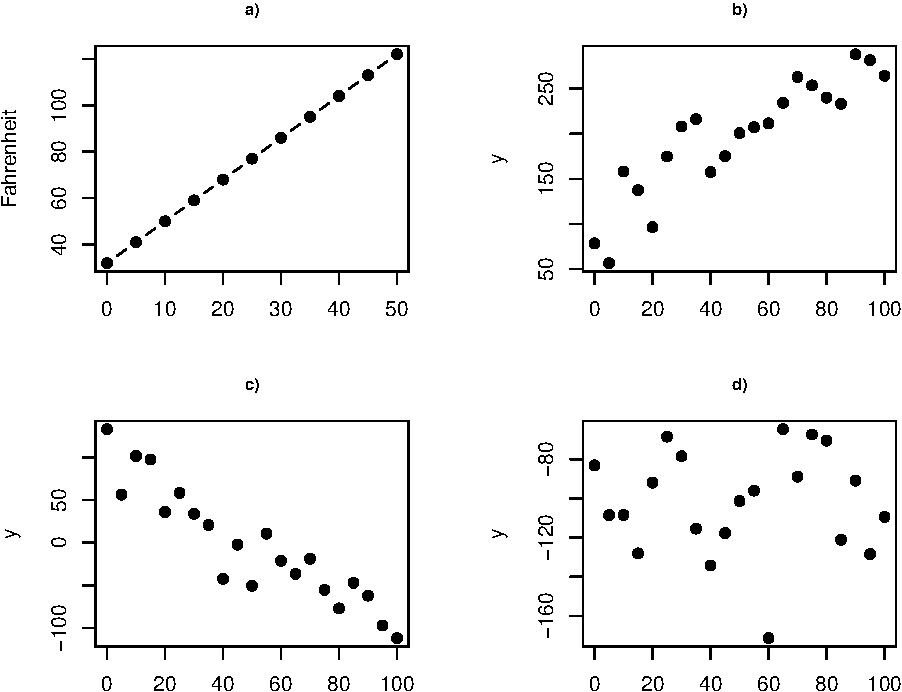
\includegraphics{session-regression-I-files/figures/fig-intro-det-vs-stat-1} 

}

\caption{Determinisitc vs. statistical relationship: a) deterministic: equation exactly describes the relationship between the two variables e.g. $Fahrenheit=9/5*Celcius+32$; b) statistical relationship between x and y is not perfect (increasing), c)  statistical relationship between x and y is not perfect (decreasing), d) random signal}\label{fig:fig-intro-det-vs-stat}
\end{figure}

\hypertarget{example-data}{%
\subsubsection{Example data}\label{example-data}}

Example data contain the body weight (kg) and plasma volume (liters) for
eight healthy men.

\begin{Shaded}
\begin{Highlighting}[]
\NormalTok{weight <-}\StringTok{ }\KeywordTok{c}\NormalTok{(}\DecValTok{58}\NormalTok{, }\DecValTok{70}\NormalTok{, }\DecValTok{74}\NormalTok{, }\FloatTok{63.5}\NormalTok{, }\FloatTok{62.0}\NormalTok{, }\FloatTok{70.5}\NormalTok{, }\FloatTok{71.0}\NormalTok{, }\FloatTok{66.0}\NormalTok{) }\CommentTok{# body weight (kg)}
\NormalTok{plasma <-}\StringTok{ }\KeywordTok{c}\NormalTok{(}\FloatTok{2.75}\NormalTok{, }\FloatTok{2.86}\NormalTok{, }\FloatTok{3.37}\NormalTok{, }\FloatTok{2.76}\NormalTok{, }\FloatTok{2.62}\NormalTok{, }\FloatTok{3.49}\NormalTok{, }\FloatTok{3.05}\NormalTok{, }\FloatTok{3.12}\NormalTok{) }\CommentTok{# plasma volume (liters)}
\end{Highlighting}
\end{Shaded}

\begin{figure}[H]

{\centering 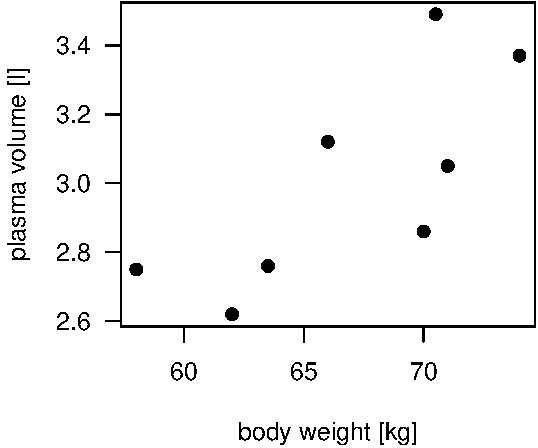
\includegraphics{session-regression-I-files/figures/fig-intro-example-1} 

}

\caption{Scatter plot of the data shows that high plasma volume tends to be associated with high weight and *vice verca*.}\label{fig:fig-intro-example}
\end{figure}

\begin{figure}[H]

{\centering 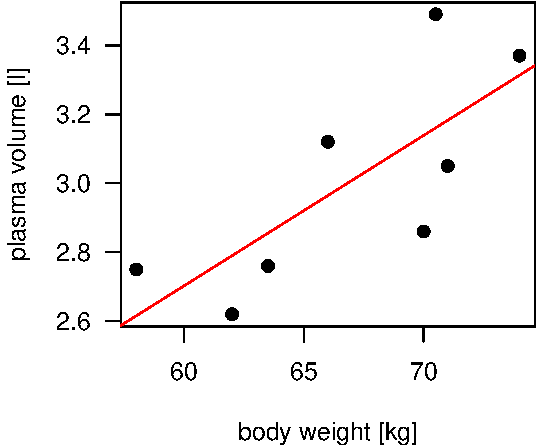
\includegraphics{session-regression-I-files/figures/fig-intro-example-reg-1} 

}

\caption{Scatter plot of the data shows that high plasma volume tends to be associated with high weight and *vice verca*. Linear regrssion gives the equation of the straight line that best describes how the outcome changes (increase or decreases) with a change of exposure variable (in red)}\label{fig:fig-intro-example-reg}
\end{figure}

The equation of the regression line is:

\[y=\beta_0 + \beta_1x\]

or mathematically using matrix notation \[Y=\beta_0 + \beta_1X\]

\begin{figure}[H]

{\centering 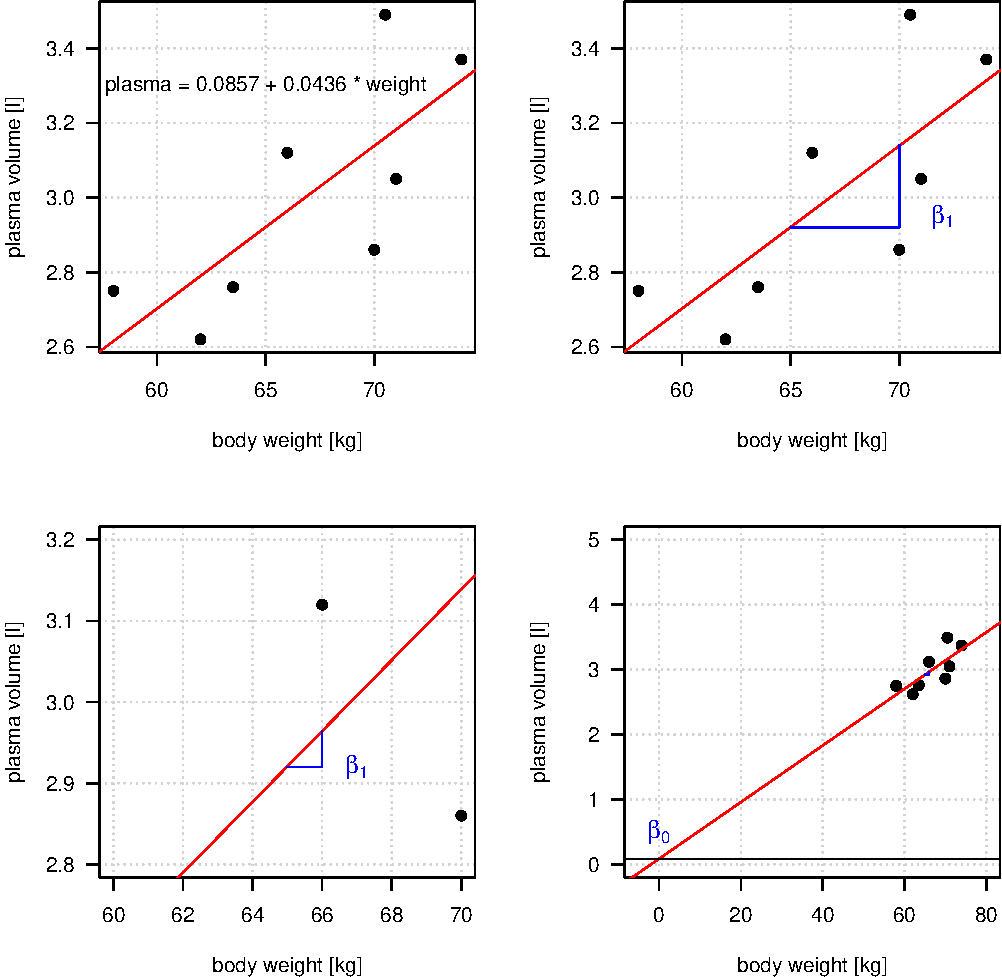
\includegraphics{session-regression-I-files/figures/fig-intro-example-reg-parameters-1} 

}

\caption{Scatter plot of the data shows that high plasma volume tends to be associated with high weight and *vice verca*. Linear regrssion gives the equation of the straight line that best describes how the outcome changes (increase or decreases) with a change of exposure variable (in red). Parameters explanation}\label{fig:fig-intro-example-reg-parameters}
\end{figure}

\hypertarget{quiz-regression-model-parameters}{%
\subsection{\texorpdfstring{\href{https://forms.gle/8jSsdQehGhjw87E38}{Quiz}:
regression model
parameters}{Quiz: regression model parameters}}\label{quiz-regression-model-parameters}}

\newpage

\hypertarget{estimating-model-coefficients}{%
\section{Estimating model
coefficients}\label{estimating-model-coefficients}}

In practice, \(\beta_0\) and \(\beta_1\) are usually unknown. The
best-fitting line is derived using the method of \textbf{least squares},
i.e.~by finding the values of the parameters \(\beta_0\) and \(\beta_1\)
tht minimize the sum of the squared vertical distances of the points
from the line.

\begin{center}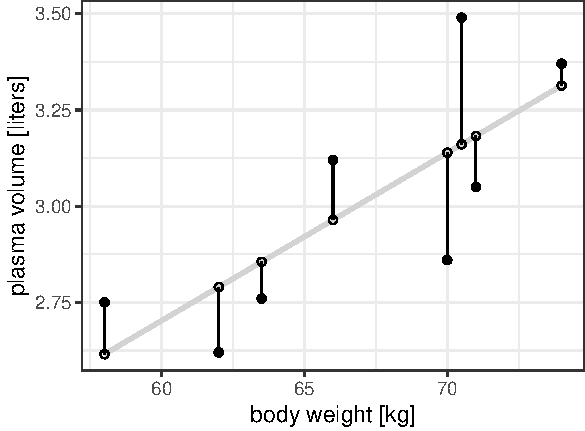
\includegraphics{session-regression-I-files/figures/coeff-residuals-1} \end{center}

Let \((x_1, y_1), (x_2, y_2), ..., (x_n, y_n)\) represent \(n\)
observation pairs, each of which consists of a measurement of \(X\) and
\(Y\), e.g.~in our example we have 8 pairs of observations, e.g. (58,
2.75), (70, 2.86) etc.

\begin{Shaded}
\begin{Highlighting}[]
\NormalTok{weight <-}\StringTok{ }\KeywordTok{c}\NormalTok{(}\DecValTok{58}\NormalTok{, }\DecValTok{70}\NormalTok{, }\DecValTok{74}\NormalTok{, }\FloatTok{63.5}\NormalTok{, }\FloatTok{62.0}\NormalTok{, }\FloatTok{70.5}\NormalTok{, }\FloatTok{71.0}\NormalTok{, }\FloatTok{66.0}\NormalTok{) }\CommentTok{# body weight (kg)}
\NormalTok{plasma <-}\StringTok{ }\KeywordTok{c}\NormalTok{(}\FloatTok{2.75}\NormalTok{, }\FloatTok{2.86}\NormalTok{, }\FloatTok{3.37}\NormalTok{, }\FloatTok{2.76}\NormalTok{, }\FloatTok{2.62}\NormalTok{, }\FloatTok{3.49}\NormalTok{, }\FloatTok{3.05}\NormalTok{, }\FloatTok{3.12}\NormalTok{) }\CommentTok{# plasma volume (liters)}
\end{Highlighting}
\end{Shaded}

We seek to find coefficients estimates \(\hat{\beta_0}\) and
\(\hat{\beta_1}\) such that liner model fits the available data well,
i.e.~such that the resulting line is as close as possible to the 8 data
points.

There are a number of ways of measuring \emph{closeness}. By far the
most common approach involves minimizing the \emph{least squares}
criterion.

Let \(\hat{y_i}=\hat{\beta_0} + \hat{\beta_1}x_i\) be the prediction
\(Y\) based on the \(i\)th value of \(X\). Then
\(\epsilon_i = y_i - \hat{y_i}\) represents the \(i\)th \emph{residual},
i.e.~the difference between the \(i\)th observed response value and the
\(i\)th response value that is predicted by the linear model.

RSS, the \emph{residual sum of squares} is defined as:
\[RSS = \epsilon_1^2 + \epsilon_2^2 + ... \epsilon_n^2\] or equivalently
as:
\[RSS=(y_1-\hat{\beta_0}-\hat{\beta_1}x_1)^2+(y_2-\hat{\beta_0}-\hat{\beta_1}x_2)^2+...+(y_n-\hat{\beta_0}-\hat{\beta_1}x_n)^2\]

The least squares approach chooses \(\hat{\beta_0}\) and
\(\hat{\beta_1}\) to minimize the RSS. With some calculus one gets:

\[\hat{\beta_1}= \frac{\sum_{i=1}^{n}(x_i-\overline{x})(y_i-\overline{y})}{\sum_{i=1}^{n}(x_i-\overline{x})^2}\]
\[\hat{\beta_0}=\overline{y}-\hat{\beta_1}\overline{x}\]

where \(\overline{y}=\frac{1}{n}\sum_{i=1}^{n}y_i\) and
\(\overline{x}=\frac{1}{n}\sum_{i=1}^{n}x_i\) are the sample means.

\href{pen-and-paper-plasma-volume.pdf}{Pen and Paper exercise}:
Estimating model coefficients

\hypertarget{hypothesis-testing}{%
\section{Hypothesis testing}\label{hypothesis-testing}}

\hypertarget{accuracy-of-the-coefficient-estimates}{%
\subsection{Accuracy of the coefficient
estimates}\label{accuracy-of-the-coefficient-estimates}}

\begin{itemize}
\tightlist
\item
  The calculated \(\hat{\beta_0}\) and \(\hat{\beta_1}\) are estimates
  of the population values of the intercept and slope and are,
  therefore, subject to sampling variation
\item
  Their precision is measure by their standard errors
  \[s.e(\hat{\beta_0})=s*\sqrt{[\frac{1}{n}+\frac{x_i^2}{\sum_{i=1}^{n}(x_i-\overline{x})^2}]}\]
  \[s.e(\hat{\beta_1})=\frac{s}{\sqrt{\sum_{i=1}^{n}(x_i-\overline{x})^2}}\]
  where, \(s\) is the \emph{standard deviation of the points about the
  line}. It has \((n-2)\) degrees of freedom, i.e.~the sample size minus
  the number of regression coefficients
  \[s=\sqrt{[\frac{\sum_{i=1}^{n}(y_i-\overline{y})^2-\overline{\beta_1}\sum_{i=1}^{n}(x_i-\overline{x})^2}{n-2}]}\]
\end{itemize}

\href{pen-and-paper-plasma-volume.pdf}{Pen and Paper exercise}: Accuracy
of the coefficient estimates

\hypertarget{confidence-interval}{%
\subsection{Confidence interval}\label{confidence-interval}}

\begin{itemize}
\tightlist
\item
  Standard errors can be used to compute \texttt{confidence\ interval}.
\item
  A 95\% confidence interval is defined as a range of values such that
  with 95\% probability, the range will contain the true unknown value
  of the parameter.
\item
  The range is defined in terms of lower and upper limits computed from
  the data. For linear regression, the 95\% confidence intervals takes
  form:
  \[[\hat{\beta_1}-2*s.e.(\hat{\beta_1}), \hat{\beta_1}+2*s.e.(\hat{\beta_1})]\]
  and
  \[[\hat{\beta_1}-2*s.e.(\hat{\beta_0}), \hat{\beta_1}+2*s.e.(\hat{\beta_0})]\]
\end{itemize}

\hypertarget{hypothesis-testing-1}{%
\subsection{Hypothesis testing}\label{hypothesis-testing-1}}

\begin{itemize}
\tightlist
\item
  Standard errors can also be used to perform
  \texttt{hypothesis\ testing} on the coefficients.
\item
  The most common hypothesis test involves testing the
  \texttt{null\ hypothesis} of: \newline
\end{itemize}

\(H_0:\) There is no relationship between \(X\) and \(Y\) \newline

versus the \texttt{alternative\ hypothesis} \newline

\(H_a:\) There is some relationship between \(X\) and \(Y\)

Mathematically, this corresponds to testing \[H_0: \beta_1=0\] versus
\[H_0: \beta_1\neq0\] since if \[\beta_1=0\] then the model
\[Y=\beta_0+\beta_1X + \epsilon\] reduces to \[Y=\beta_0 + \epsilon\]

To test the null hypothesis we need to determine whether
\(\hat{\beta_1}\), our estimate of \(\beta_1\), is sufficiently far from
zero that we can be confident that \(\beta_1\) is non-zero.

How far is far enough? This depends on the accuracy of
\(\hat{\beta_1}\), that is standard error \(s.e.(\hat{\beta_1})\). If
\(s.e.(\hat{\beta_1})\) is small, then small values of \(\hat{\beta_1}\)
may provide strong evidence that \(\hat{\beta_1}\neq0\) and \emph{vice
verca}. In practice, we compute a \texttt{t-statistics} given by
\[t=\frac{\hat{\beta_1}-0}{s.e.(\hat{\beta_1})}\] which measures the
standard deviations that \(\hat{\beta_1}\) is away from 0.

If there really is no relationship between \(X\) and \(Y\), then we this
will have a \(t\)-distribution with \(n-2\) degrees of freedom. From
previous sessions, we now know how to compute probability of observing
any value equal to \(|t|\). We call this probability the \(p-value\).

We can interpret the \(p-value\) as follows: a small p-value indicates
that it is unlikely to observe such a substantial association between
\(X\) and \(Y\) due to chance, i.e.~in the absence of any real
association. We therefore can \texttt{reject\ the\ null\ hypothesis}.

Typical p-value cutoffs for rejecting the null hypothesis are 5 or 1\%.

\href{pen-and-paper-plasma-volume.pdf}{Pen and Paper exercise}:
Hypothesis testing

\hypertarget{live-coding-demo}{%
\subsection{Live coding demo}\label{live-coding-demo}}

\begin{Shaded}
\begin{Highlighting}[]
\CommentTok{# Data}
\NormalTok{weight <-}\StringTok{ }\KeywordTok{c}\NormalTok{(}\DecValTok{58}\NormalTok{, }\DecValTok{70}\NormalTok{, }\DecValTok{74}\NormalTok{, }\FloatTok{63.5}\NormalTok{, }\FloatTok{62.0}\NormalTok{, }\FloatTok{70.5}\NormalTok{, }\FloatTok{71.0}\NormalTok{, }\FloatTok{66.0}\NormalTok{)}
\NormalTok{plasma <-}\StringTok{ }\KeywordTok{c}\NormalTok{(}\FloatTok{2.75}\NormalTok{, }\FloatTok{2.86}\NormalTok{, }\FloatTok{3.37}\NormalTok{, }\FloatTok{2.76}\NormalTok{, }\FloatTok{2.62}\NormalTok{, }\FloatTok{3.49}\NormalTok{, }\FloatTok{3.05}\NormalTok{, }\FloatTok{3.12}\NormalTok{) }

\CommentTok{# Plot}
\KeywordTok{plot}\NormalTok{(weight, plasma)}

\CommentTok{# Regression}
\NormalTok{reg <-}\StringTok{ }\KeywordTok{lm}\NormalTok{(plasma}\OperatorTok{~}\NormalTok{weight)}
\KeywordTok{summary}\NormalTok{(reg)}

\CommentTok{# Coefficients}
\KeywordTok{coef}\NormalTok{(reg)}

\CommentTok{# Confidence intervals}
\KeywordTok{confint}\NormalTok{(reg)}

\CommentTok{# Add regression line to the plot}
\KeywordTok{abline}\NormalTok{(reg)}
\end{Highlighting}
\end{Shaded}

\begin{figure}[H]

{\centering 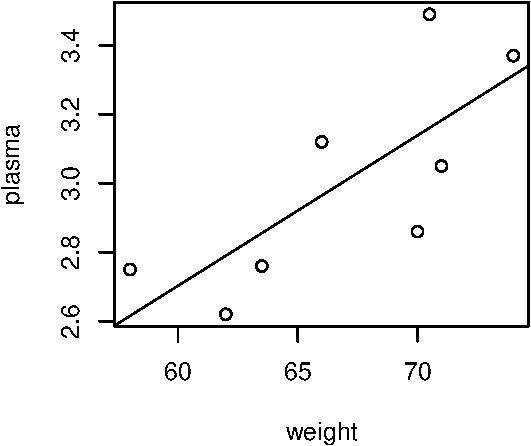
\includegraphics{session-regression-I-files/figures/unnamed-chunk-3-1} 

}

\caption{Body weight vs. plasma volume}\label{fig:unnamed-chunk-3}
\end{figure}

\begin{verbatim}
## 
## Call:
## lm(formula = plasma ~ weight)
## 
## Residuals:
##      Min       1Q   Median       3Q      Max 
## -0.27880 -0.14178 -0.01928  0.13986  0.32939 
## 
## Coefficients:
##             Estimate Std. Error t value Pr(>|t|)  
## (Intercept)  0.08572    1.02400   0.084   0.9360  
## weight       0.04362    0.01527   2.857   0.0289 *
## ---
## Signif. codes:  0 '***' 0.001 '**' 0.01 '*' 0.05 '.' 0.1 ' ' 1
## 
## Residual standard error: 0.2188 on 6 degrees of freedom
## Multiple R-squared:  0.5763, Adjusted R-squared:  0.5057 
## F-statistic:  8.16 on 1 and 6 DF,  p-value: 0.02893
## 
## (Intercept)      weight 
##  0.08572428  0.04361534 
##                    2.5 %     97.5 %
## (Intercept) -2.419908594 2.59135716
## weight       0.006255005 0.08097567
\end{verbatim}

\hypertarget{prediction}{%
\section{Prediction}\label{prediction}}

Sometimes it may be useful to use the regression equation to predict the
value of \(y_i\) for a particular value of \(x_i\), say \(x_i´\). The
\texttt{predicted\ value} is: \[y_i'=\hat{\beta_0}+\hat{\beta_1}x_i'\]
and its standard error is:
\[s.e.(y_i')=s\sqrt{[1+\frac{1}{n}+\frac{(x_i-\overline{x_i})^2}{\sum_{i=1}^{n}(x_i-\overline{x_i})^2}]}\]

The standard error is least when \(x_i´\) is close to the mean,
\(\overline{x}\)

In general, one should be reluctant to use the regression line for
predicting values outside the range of \(x\) in the original data, as
the linear relationship will not necessarily hold true beyond the range
over which it has been fitted.

\hypertarget{prediction-interval}{%
\subsection{Prediction interval}\label{prediction-interval}}

There is also a concept called \texttt{prediction\ interval}. Here, we
look at any specific value of \(x_i\), and find an interval around the
predicted value \(y_i'\) for \(x_i\) such that there is a 95\%
probability that the real value of y (in the population) corresponding
to \(x_i\) is within this interval.

Prediction interval regression vs.~confidence interval

\begin{itemize}
\tightlist
\item
  95\% confidence interval: there is 95\% probability that the true best
  fit-line for the population lies within the confidence interval
\item
  95\% prediction interval: 95\% of the \(y\) values found for a certain
  \(x\) value will be within the interval range around the linear
  regression line
\item
  prediction interval \(>\) than a confidence interval, as it must
  account for both the uncertainty in knowing the value of the
  population mean, plus data scatter.
\end{itemize}

The 95\% prediction interval of the forecasted value \(y_i'\):

\hypertarget{live-coding-demo-1}{%
\subsection{Live coding demo}\label{live-coding-demo-1}}

\begin{Shaded}
\begin{Highlighting}[]
\CommentTok{# Prediction}
\KeywordTok{predict}\NormalTok{(reg, }\KeywordTok{data.frame}\NormalTok{(}\DataTypeTok{weight=}\DecValTok{60}\NormalTok{))}
\end{Highlighting}
\end{Shaded}

\begin{verbatim}
##        1 
## 2.702645
\end{verbatim}

\begin{Shaded}
\begin{Highlighting}[]
\KeywordTok{predict}\NormalTok{(reg, }\KeywordTok{data.frame}\NormalTok{(}\DataTypeTok{weight=}\KeywordTok{c}\NormalTok{(}\DecValTok{60}\NormalTok{, }\DecValTok{70}\NormalTok{)))}
\end{Highlighting}
\end{Shaded}

\begin{verbatim}
##        1        2 
## 2.702645 3.138798
\end{verbatim}

\begin{Shaded}
\begin{Highlighting}[]
\CommentTok{# Prediction with confidence intervals}
\KeywordTok{predict}\NormalTok{(reg, }\KeywordTok{data.frame}\NormalTok{(}\DataTypeTok{weight=}\DecValTok{66}\NormalTok{), }\DataTypeTok{interval=}\StringTok{"prediction"}\NormalTok{)}
\end{Highlighting}
\end{Shaded}

\begin{verbatim}
##        fit      lwr      upr
## 1 2.964337 2.395511 3.533162
\end{verbatim}

\hypertarget{asesssing-the-accuracy-of-the-model-correlation}{%
\section{Asesssing the Accuracy of the Model \&
Correlation}\label{asesssing-the-accuracy-of-the-model-correlation}}

Once we have rejected the null hypothesis (\(H_0:\)there is no
relationship between X and Y) in favor of the alternative hypothesis
(\(H_a\)there is some relationship between X and Y) we may want to
quantify \texttt{the\ extent\ to\ which\ the\ model\ fits\ the\ data}.

The quality of a linear regression fit is typically assessed using two
related quantities: - RSE, the residual standard error - \(R^2\)
statistics

\hypertarget{rse-residual-standard-error}{%
\subsection{RSE, Residual standard
error}\label{rse-residual-standard-error}}

\begin{itemize}
\tightlist
\item
  RSE is a measure of \texttt{lack\ of\ fit} of the model to the data
\item
  It is measured in units of \(Y\).
\end{itemize}

Going back to linear regression model, and writing it in the formal
complete way: \[Y=\beta_0+\beta_1X+\epsilon\] we can see that each
observation is associated with an error term \(\epsilon\). This means
that even knowing \(\beta_0\) and \(\beta_1\) one cannot perfectly
predict \(Y\) from \(X\).

\texttt{RSE} is an estimate of the standard deviation of \(\epsilon\),
that can be viewed as the average amount that the response will deviate
from the true regression line. It is calculated
\[RSE=\sqrt{\frac{1}{n-2}RSS} = \sqrt{\frac{1}{n-2}\sum_{i=1}{n}(y_i-\hat{y_i})^2}\]
where \[RSE=\sum_{i=1}^{n}(y_i-\hat{y_i})^2\]

\begin{figure}[H]

{\centering 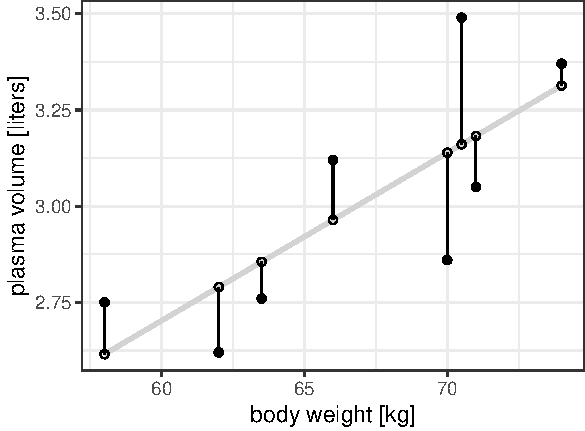
\includegraphics{session-regression-I-files/figures/rse-1} 

}

\end{figure}

\hypertarget{live-coding-demo-2}{%
\subsubsection{Live coding demo}\label{live-coding-demo-2}}

\begin{Shaded}
\begin{Highlighting}[]
\CommentTok{#weight <- c(58, 70, 74, 63.5, 62.0, 70.5, 71.0, 66.0) # body weight (kg)}
\CommentTok{#plasma <- c(2.75, 2.86, 3.37, 2.76, 2.62, 3.49, 3.05, 3.12) # plasma volume (liters)}

\NormalTok{plasma}
\end{Highlighting}
\end{Shaded}

\begin{verbatim}
## [1] 2.75 2.86 3.37 2.76 2.62 3.49 3.05 3.12
\end{verbatim}

\begin{Shaded}
\begin{Highlighting}[]
\NormalTok{weight }
\end{Highlighting}
\end{Shaded}

\begin{verbatim}
## [1] 58.0 70.0 74.0 63.5 62.0 70.5 71.0 66.0
\end{verbatim}

\begin{Shaded}
\begin{Highlighting}[]
\KeywordTok{head}\NormalTok{(data.reg)}
\end{Highlighting}
\end{Shaded}

\begin{verbatim}
##   plasma weight predicted   residuals
## 1   2.75   58.0  2.615414  0.13458612
## 2   2.86   70.0  3.138798 -0.27879793
## 3   3.37   74.0  3.313259  0.05674072
## 4   2.76   63.5  2.855298 -0.09529823
## 5   2.62   62.0  2.789875 -0.16987523
## 6   3.49   70.5  3.160606  0.32939440
\end{verbatim}

\begin{Shaded}
\begin{Highlighting}[]
\NormalTok{reg <-}\StringTok{ }\KeywordTok{lm}\NormalTok{(data.reg}\OperatorTok{$}\NormalTok{plasma}\OperatorTok{~}\NormalTok{data.reg}\OperatorTok{$}\NormalTok{weight)}

\CommentTok{# predict Y given the values of X and regression model reg}
\NormalTok{y.pred <-}\StringTok{ }\KeywordTok{predict}\NormalTok{(reg, }\KeywordTok{data.frame}\NormalTok{(}\DataTypeTok{weight=}\NormalTok{data.reg}\OperatorTok{$}\NormalTok{weight))}
\NormalTok{y.pred}
\end{Highlighting}
\end{Shaded}

\begin{verbatim}
##        1        2        3        4        5        6        7        8 
## 2.615414 3.138798 3.313259 2.855298 2.789875 3.160606 3.182413 2.964337
\end{verbatim}

\begin{Shaded}
\begin{Highlighting}[]
\CommentTok{# calculate residuals}
\NormalTok{e.terms <-}\StringTok{ }\NormalTok{data.reg}\OperatorTok{$}\NormalTok{plasma}\OperatorTok{-}\NormalTok{y.pred}
\NormalTok{e.terms}
\end{Highlighting}
\end{Shaded}

\begin{verbatim}
##           1           2           3           4           5           6 
##  0.13458612 -0.27879793  0.05674072 -0.09529823 -0.16987523  0.32939440 
##           7           8 
## -0.13241327  0.15566342
\end{verbatim}

\begin{Shaded}
\begin{Highlighting}[]
\CommentTok{# calculate RSS}
\NormalTok{RSS=}\KeywordTok{sum}\NormalTok{(e.terms}\OperatorTok{^}\DecValTok{2}\NormalTok{)}

\CommentTok{# calculate RSE}
\NormalTok{n=}\KeywordTok{nrow}\NormalTok{(data.reg)}
\NormalTok{RSE <-}\StringTok{ }\KeywordTok{sqrt}\NormalTok{((}\DecValTok{1}\OperatorTok{/}\NormalTok{(n}\DecValTok{-2}\NormalTok{))}\OperatorTok{*}\NormalTok{RSS)}

\CommentTok{# R reg objects contains it all}
\KeywordTok{names}\NormalTok{(reg)}
\end{Highlighting}
\end{Shaded}

\begin{verbatim}
##  [1] "coefficients"  "residuals"     "effects"       "rank"         
##  [5] "fitted.values" "assign"        "qr"            "df.residual"  
##  [9] "xlevels"       "call"          "terms"         "model"
\end{verbatim}

\begin{Shaded}
\begin{Highlighting}[]
\NormalTok{reg}\OperatorTok{$}\NormalTok{fitted.values}
\end{Highlighting}
\end{Shaded}

\begin{verbatim}
##        1        2        3        4        5        6        7        8 
## 2.615414 3.138798 3.313259 2.855298 2.789875 3.160606 3.182413 2.964337
\end{verbatim}

\begin{Shaded}
\begin{Highlighting}[]
\NormalTok{reg}\OperatorTok{$}\NormalTok{residuals}
\end{Highlighting}
\end{Shaded}

\begin{verbatim}
##           1           2           3           4           5           6 
##  0.13458612 -0.27879793  0.05674072 -0.09529823 -0.16987523  0.32939440 
##           7           8 
## -0.13241327  0.15566342
\end{verbatim}

\begin{Shaded}
\begin{Highlighting}[]
\CommentTok{# RSE}
\KeywordTok{summary}\NormalTok{(reg)}
\end{Highlighting}
\end{Shaded}

\begin{verbatim}
## 
## Call:
## lm(formula = data.reg$plasma ~ data.reg$weight)
## 
## Residuals:
##      Min       1Q   Median       3Q      Max 
## -0.27880 -0.14178 -0.01928  0.13986  0.32939 
## 
## Coefficients:
##                 Estimate Std. Error t value Pr(>|t|)  
## (Intercept)      0.08572    1.02400   0.084   0.9360  
## data.reg$weight  0.04362    0.01527   2.857   0.0289 *
## ---
## Signif. codes:  0 '***' 0.001 '**' 0.01 '*' 0.05 '.' 0.1 ' ' 1
## 
## Residual standard error: 0.2188 on 6 degrees of freedom
## Multiple R-squared:  0.5763, Adjusted R-squared:  0.5057 
## F-statistic:  8.16 on 1 and 6 DF,  p-value: 0.02893
\end{verbatim}

\hypertarget{r2-statistics}{%
\subsection{\texorpdfstring{\(R^2\)
statistics}{R\^{}2 statistics}}\label{r2-statistics}}

\begin{itemize}
\tightlist
\item
  \(R^2\) statistics is an alternative measure of fit and measure of
  linear relationship between \(X\) and \(Y\)
\item
  It takes the form of a proportion, the proportion of variance
  explained, hence is independent of the scale of \(Y\)
\item
  \(0 \leq R^2 \leq 1\)
\end{itemize}

\[R^2=\frac{TSS-RSS}{TSS}=1-\frac{RSS}{TSS}\] where
\[TSS=\sum_{i=1}^{n}(y_i-\overline{y})\]

\hypertarget{correlation}{%
\subsection{Correlation}\label{correlation}}

\begin{itemize}
\tightlist
\item
  is also a measure of linear regression between \(X\) and \(Y\)
  \[Cor(X,Y)=\frac{\sum_{i=1}^{n}(x_i-\overline{x})(y_i-\overline{y})}{\sqrt{\sum_{i=1}^{n}(x_i-\overline{x})^2}\sqrt{\sum_{i=1}^{n}(y_i-\overline{y})^2}}\]
\end{itemize}

This suggests that we should be able to use \(r=Cor(X,Y)\) to assess the
fit of the linear model

In fact, For simple linear regression, it can be shown that \[R^2=r^2\]

\hypertarget{live-coding-demo-3}{%
\subsubsection{Live coding demo}\label{live-coding-demo-3}}

\begin{Shaded}
\begin{Highlighting}[]
\CommentTok{#summary(reg)}
\KeywordTok{names}\NormalTok{(reg)}
\end{Highlighting}
\end{Shaded}

\begin{verbatim}
##  [1] "coefficients"  "residuals"     "effects"       "rank"         
##  [5] "fitted.values" "assign"        "qr"            "df.residual"  
##  [9] "xlevels"       "call"          "terms"         "model"
\end{verbatim}

\begin{Shaded}
\begin{Highlighting}[]
\NormalTok{r2 <-}\StringTok{ }\KeywordTok{cor}\NormalTok{(data.reg}\OperatorTok{$}\NormalTok{plasma, data.reg}\OperatorTok{$}\NormalTok{weight)}\OperatorTok{^}\DecValTok{2}
\end{Highlighting}
\end{Shaded}

\hypertarget{assumptions}{%
\section{Assumptions}\label{assumptions}}

\begin{itemize}
\tightlist
\item
  The regression model is linear in parameters, i.e.~the true
  relationship is linear
\item
  Errors, \(\epsilon_i\), are independent
\item
  Errors, \(\epsilon_i\), at each value of predictor, \(x_i\), are
  normally distributed
\item
  Errors, \(\epsilon_i\), at each value of predictor, \(x_i\), have
  equal variances, \(\sigma^2\) (homoscedasticity of errors)
\end{itemize}

The residuals provide information about the noise term in the model, and
allow limited checks on model assumptions. Note that in small data set,
departures from assumptions may be hard to detect.

\begin{itemize}
\tightlist
\item
  A plot of residuals versus fitted values allows a visual check for any
  pattern in the residuals that might suggest a curve rather than a line
\item
  A normal probability plot of residuals: if residuals are from a normal
  distribution points should like, to within statistical error, close to
  a
\end{itemize}

\hypertarget{live-coding-demo-4}{%
\subsection{Live coding demo}\label{live-coding-demo-4}}

\begin{Shaded}
\begin{Highlighting}[]
\KeywordTok{par}\NormalTok{(}\DataTypeTok{mfrow=}\KeywordTok{c}\NormalTok{(}\DecValTok{1}\NormalTok{,}\DecValTok{2}\NormalTok{))}
\KeywordTok{plot}\NormalTok{(reg, }\DataTypeTok{which=}\DecValTok{1}\OperatorTok{:}\DecValTok{2}\NormalTok{)}
\end{Highlighting}
\end{Shaded}

\begin{figure}[H]

{\centering 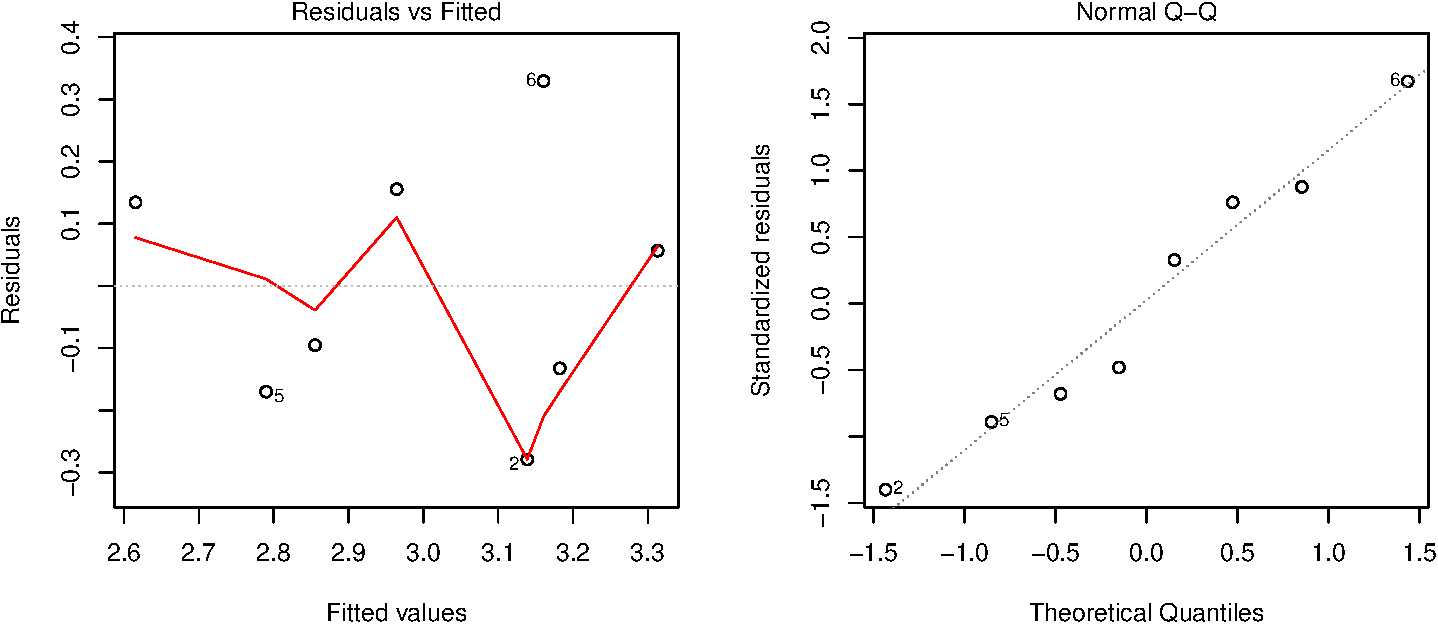
\includegraphics{session-regression-I-files/figures/unnamed-chunk-7-1} 

}

\caption{Diagnostic plots for the regression}\label{fig:unnamed-chunk-7}
\end{figure}

\hypertarget{beyond}{%
\section{Beyond}\label{beyond}}

\begin{itemize}
\tightlist
\item
  \href{https://newonlinecourses.science.psu.edu/stat501/node/286/}{Linear
  regression, ANOVA and t-test relationship}
\item
  \href{https://newonlinecourses.science.psu.edu/stat501/node/286/}{Outliers
  and influential observations} (best to read after multiple regression
  session)
\item
  \href{https://newonlinecourses.science.psu.edu/stat501/node/318/}{Data
  transformations}
\item
  \href{http://www.rwdc2.com/files/rafa.pdf}{Linear models chapter to
  dig more into mathematics behind lm}
\end{itemize}


\end{document}
